% written by Akmal Zuhdy Prasetya (H071191035)

\documentclass[peerreview]{IEEEtran}
\usepackage{cite} % Tidies up citation numbers.
\usepackage{url} % Provides better formatting of URLs.
\usepackage[utf8]{inputenc} % Allows Turkish characters.
\usepackage{gensymb}
\usepackage{amsmath}
\usepackage{amssymb}
\usepackage{booktabs} % Allows the use of \toprule, \midrule and \bottomrule in tables for horizontal lines
\usepackage{graphicx}
\usepackage{float}
\usepackage{adjustbox}
\usepackage{hyperref}
\hypersetup{
    colorlinks=true,
    linkcolor=black,
    filecolor=magenta,      
    urlcolor=cyan,
    citecolor=black,
    pdfpagemode=FullScreen,
    }

\urlstyle{same}
\usepackage[justification=centering]{caption}
\usepackage{listings} %for listings of the source code
\lstset{
  inputencoding=latin1,
  basicstyle=\footnotesize\ttfamily,
  keywordstyle=\color{blue},         
  breaklines=true, 
  showtabs=false,
  showstringspaces=false
}
\hyphenation{op-tical net-works semi-conduc-tor} % Corrects some bad hyphenation

\graphicspath{{images/}}

\begin{document}
%\begin{titlepage}
% paper title
% can use linebreaks \\ within to get better formatting as desired
\title{CycleGAN Model Implementation Report Using Tensorflow - UNHAS Final Test Project}


% author names and affiliations

\author{Akmal Zuhdy Prasetya \\
Information Systems Study Program \\
Department of Mathematics \\
Hasanuddin University\\
}
\date{6/17/22}

% make the title area
\maketitle
\tableofcontents
\listoffigures
\listoftables
%\end{titlepage}

\IEEEpeerreviewmaketitle
\begin{abstract}
Image-to-image translation is an important topic in the field of computer vision. It aims to learn the mapping between input image and output image by training the datasets, and finally translates the image style from one domain to another. In terms of the form of translation, it can be divided into the translation between two domains and multiple domains from different datasets. And it is also divided into pairs and unpaired by the training datasets. As a successful representation of the translation of an unpaired image between two domains, the CycleGAN model is of great significance to the research and application. Starting from the application background of the CycleGAN model, this paper attempts to show an implementation of CycleGAN using Tensorflow to try transforming some images into another style so we can better understand how CycleGAN works.

\end{abstract}


% INTRODUCTION
\section{Introduction}

Since the arrival of Convolutional Neural network (CNN), deep learning as an implementation algorithm of machine learning, has been widely used in Computer Vision field, from the beginning of the recognition of handwritten, object tracking, speech recognition, face recognition, and through training of fruit images dataset, help person determine the type of fruit when given image about it, until Alpha Go, it is the first computer program to defeat a professional human Go player, the first program to defeat a Go world champion, and arguably the strongest Go player in history, making the deep reinforcement learning attracted more and more researcher's attention.

At the same time, the famous model GAN (Generative Adversarial Networks) proposed by Goodfellow in 2014 \cite{goodfellow2014generative}, which is considered to be the coolest idea in the field of machine learning in the past 20 years and bring new breakthroughs to the deep learning model. The key to GAN's success is the idea of an adversarial loss that forces the generated images to be, in principle, indistinguishable from real photos. This loss is particularly powerful for image generation tasks, as this is exactly the objective that many of computer graphics aims to optimize \cite{zhu2019brief}.


% PROBLEM DEFINITION
\section{Problem Definition}
In this technical report, I focus on reproducing an implementation of CycleGAN model to translate or transform a some images into another style using Tensorflow to better understand how CycleGAN works.


% MODEL EXPLANATION
\section{CycleGAN Architecture}
In this section, we first briefly review the principle of CycleGAN and then give a comparison with the Pix2Pix GAN model image-to-image translation models.

\subsection{Background of CycleGAN}
The task of image style translation is to change a particular aspect of a given image to another, that is to say, given any two unordered image collections X and Y, the algorithm learns to automatically “translate” an image from one into the other and vice versa, which can be divided into two situations which is one is paired translation and the other is unpaired translation \cite{upadhyay2021uncertainty}.

\begin{figure}[H]
    \centering
    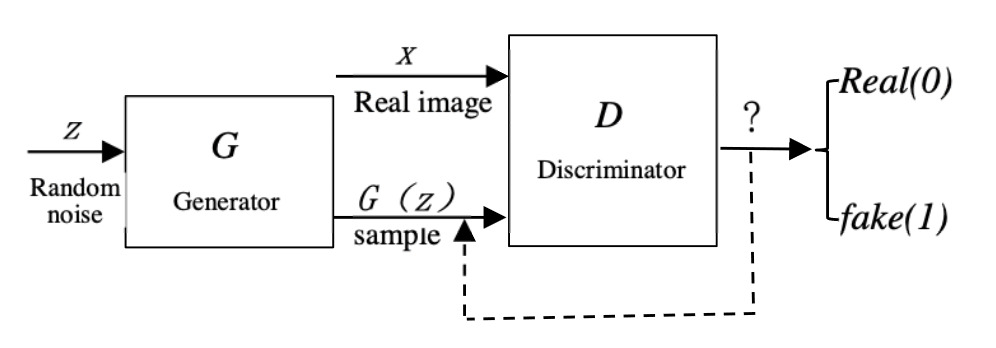
\includegraphics[width=0.8\columnwidth]{GAN Model}
    \caption{GAN model}
    \label{fig:s=gan_model}
\end{figure}

For image translation in pairs, the commonly used models is Pix2Pix \cite{isola2017image}, it can verify by example that pix2pix model has a certain universality, but also has certain limitation. First of all, the requirements of the training dataset of training samples must be in pairs, but in real life, if we want to collect a large number of data in pairs, it is a little difficulty. If the data quantity is little, and there will be a fitting, model training effect. Secondly, the image transfer achieved by this model is only limited to the transformation of different styles of the same image, such as color changes. At this time, how to use samples with different styles for training to complete the translation of image style is the basic design idea of CycleGAN model.

\subsection{CycleGAN Model Review}
As one of the most interesting and important deep learning achievements in 2017, CycleGAN has many application in the past two years. The original schematic and formula of the CycleGAN paper are as follows.

\begin{figure}[H]
    \centering
    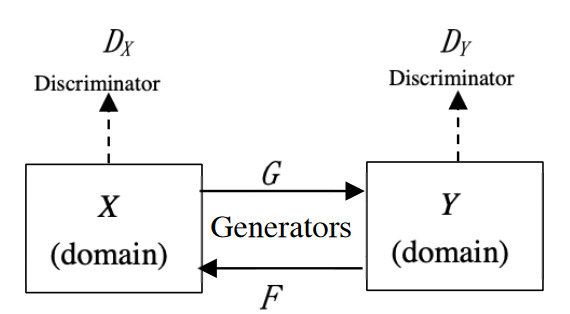
\includegraphics[width=0.8\columnwidth]{CycleGAN Model}
    \caption{CycleGAN model}
    \label{fig:s=cyclegan_model}
\end{figure}

Jun-Yan Zhun \cite{zhu2017unpaired} given two datasets $\{x_i\}(i=1$ to $M)$ and $\{y\}(j=1$ to $N)$, collected from two different domains $X$ and $Y$, where $x_i \in X$ and $y_j \in Y$, the goal of CycleGAN is to learn a mapping function: $G:X \to Y$, such that the distribution of images from $G(X)$ is distinguishable from the distribution $Y$ using adversarial loss.

CycleGAN contains two mapping functions $G:X \to Y$ and $F:Y \to X$. Two adverasial discriminators $D_X$ and $D_Y$ are proposed to distinguish whether images are translated from another domain. CycleGan applies the GAN framework to train the generative and discriminative models jointly. The overall CycelGAN loss function is expressed as follows: 

\begin{equation}
    \begin{split}
         V(G, F, D_X, D_Y) & = V_{GAN}(D_Y, G, X, Y) \\
         & + V_{GAN}(D_X, F, Y, X) \\
         & + \lambda V_{cyc}(G, F)
    \end{split}
\end{equation}

Where $V_{GAN}(D_Y, G, X, Y)$ and $V_{GAN}(D_X, F, Y, X)$ are the loss function for mapping functions $G$ and $F$, and for the discriminators $D_Y$ and $D_X$ is the cycle consistency loss that forces $F(G(x)) \approx x$ and $G(F(y)) \approx y$, in which each image can be reconstructed after a cycle mapping.$\lambda$ penalizes the importance between $V_{GAN}$ and $V_{cyc}$.

Transferring characteristics from one image to another is an exciting proposition. How cool would it be if we could take a photo and convert it into the style of Van Gogh or Picasso!

\begin{figure}[H]
    \centering
    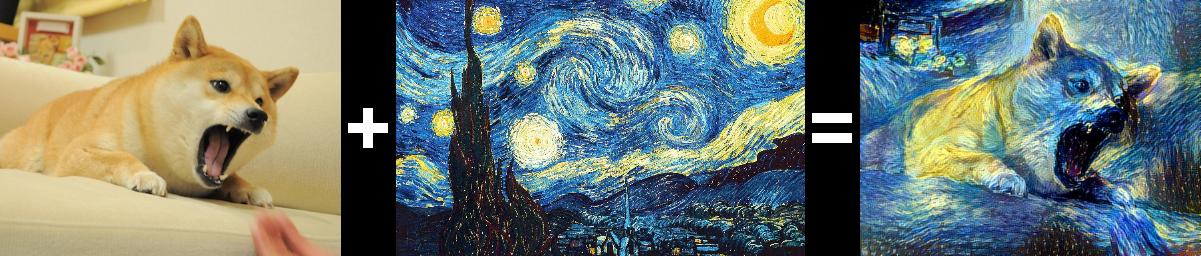
\includegraphics[width=0.8\columnwidth]{doge_starrynight}
    \caption{Image translation example 1}
    \label{fig:s=doge_starry}
\end{figure}

Or maybe we want to put a smile on Agent 42's face with the virally popular Faceapp.

\begin{figure}[H]
    \centering
    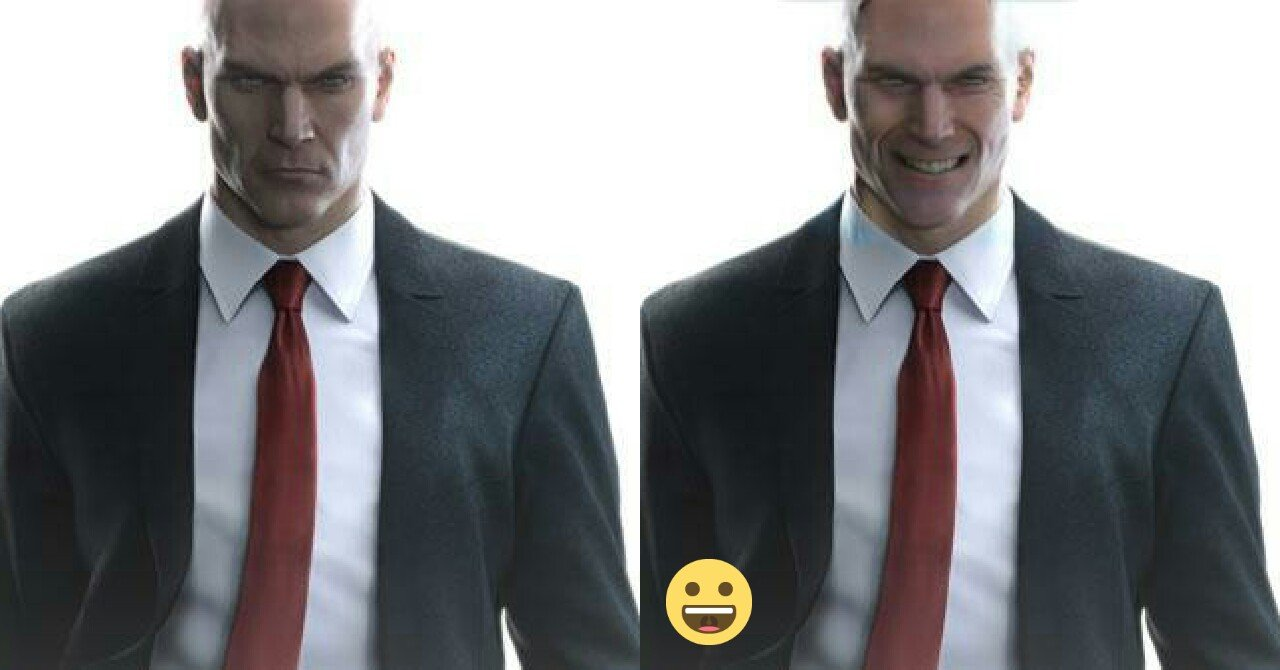
\includegraphics[width=0.8\columnwidth]{agent47}
    \caption{Image translation example 2}
    \label{fig:s=agent47}
\end{figure}

These are examples of cross domain image transfer, we want to take an image from an input domain $D_i$ Di and then transform it into an image of target domain $D_t$ without necessarily having a one-to-one mapping between images from input to target domain in the training set. Relaxation of having one-to-one mapping makes this formulation quite powerful the same method could be used to tackle a variety of problems by varying the input-output domain pairs performing artistic style transfer, adding bokeh effect to phone camera photos, creating outline maps from satellite images or convert horses to zebras and vice versa!! This is achieved by a type of generative model, specifically a Generative Adversarial Network dubbed CycleGAN. Here are some examples of what CycleGAN can do.

\begin{figure}[H]
    \centering
    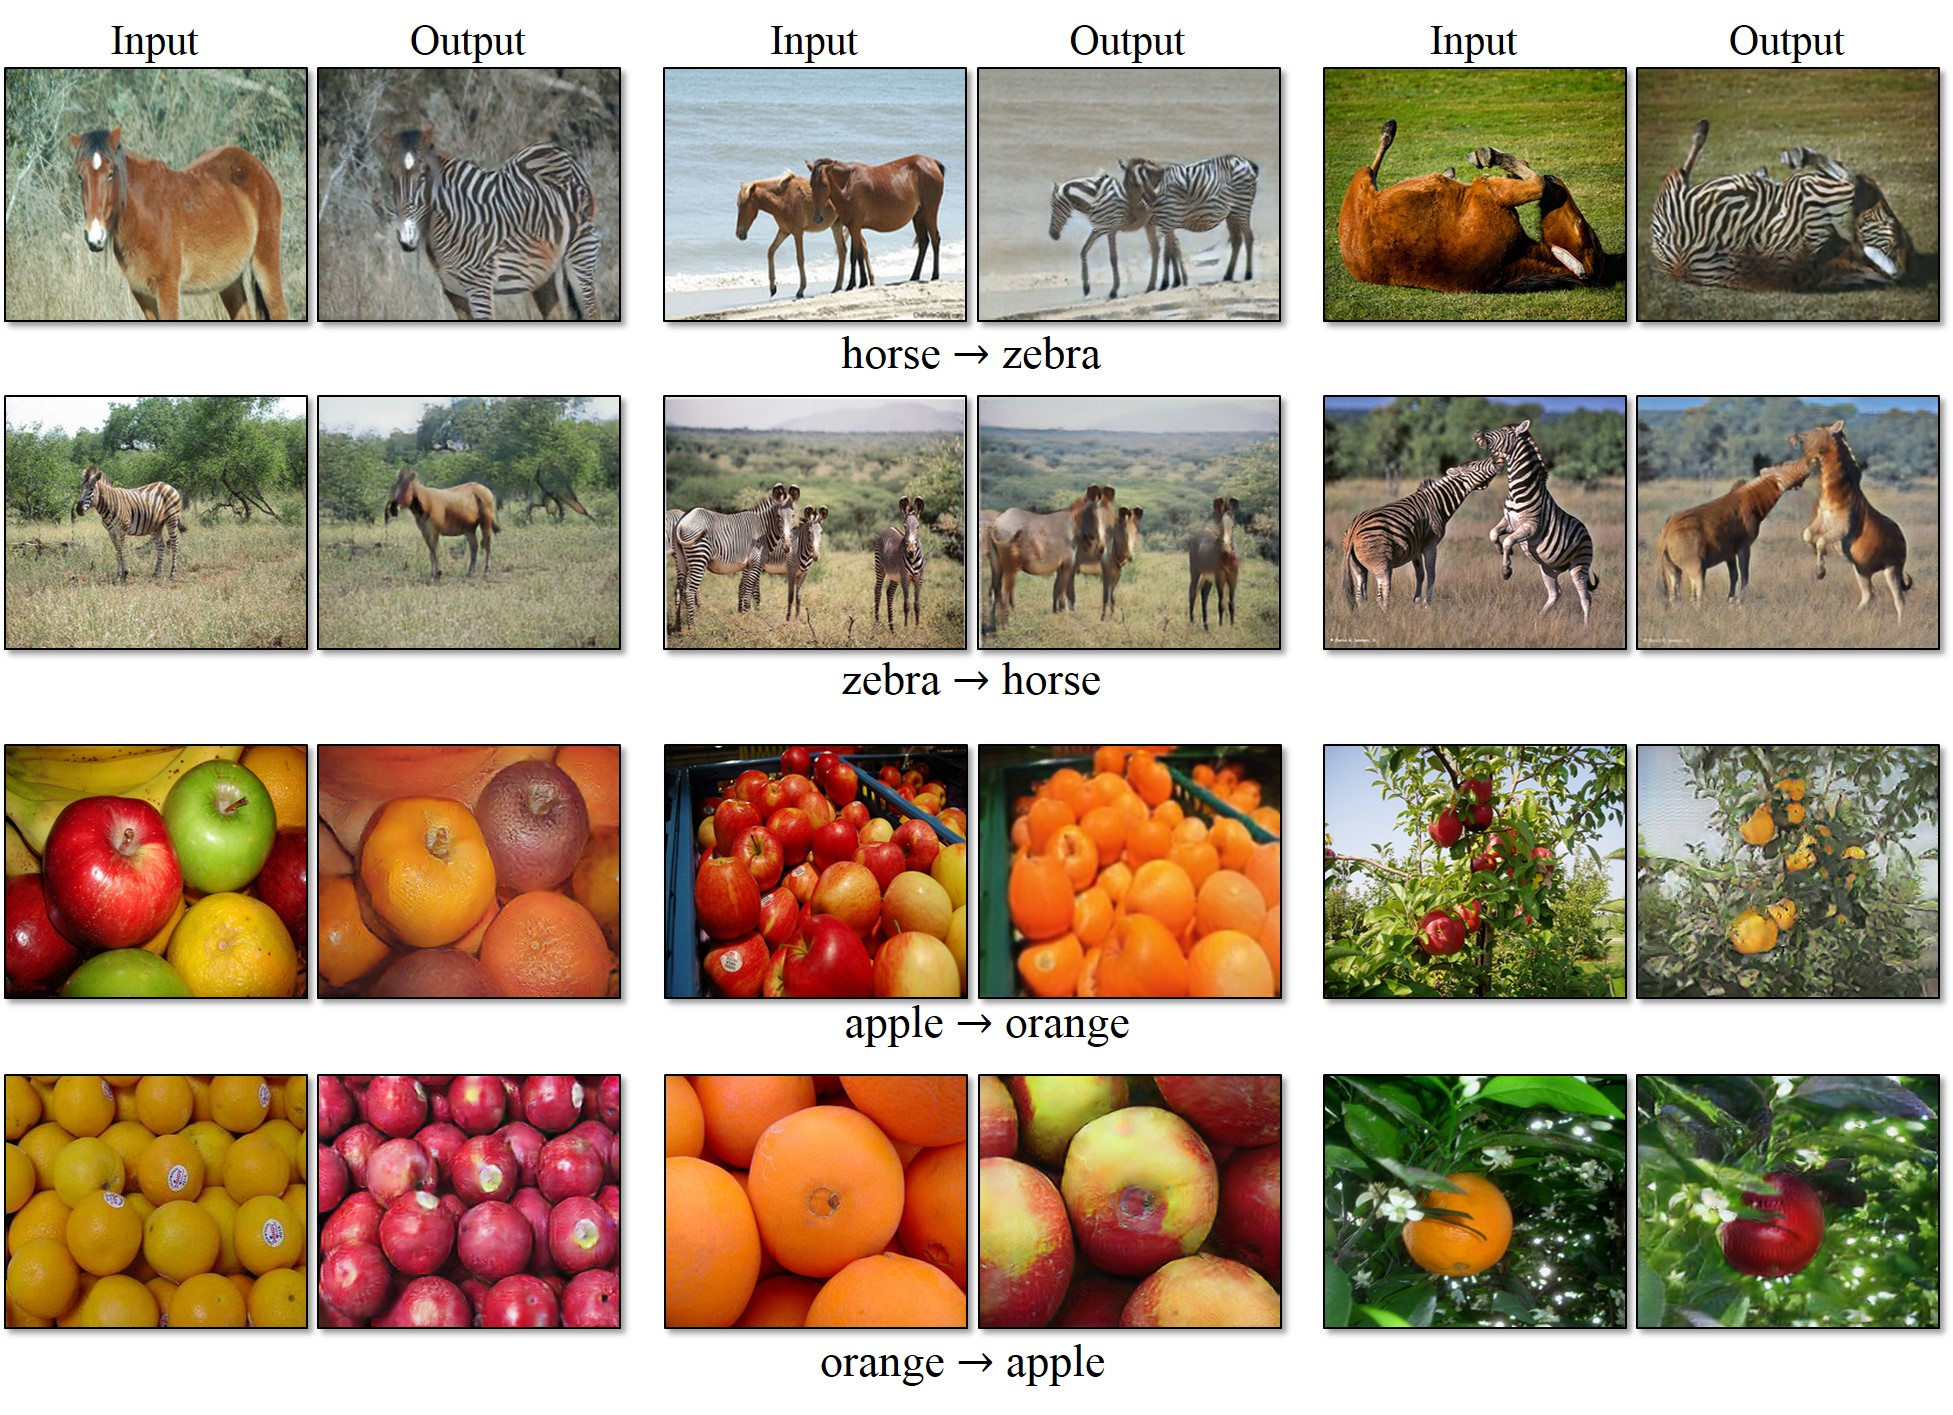
\includegraphics[width=0.8\columnwidth]{gan_example.jpg}
    \caption{CycleGAN image transformation example}
    \label{fig:s=cyclegan_example}
\end{figure}

\subsection{Unpaired Image-to-Image Translation}
As mentioned earlier, the CycleGAN works without paired examples of transformation from source to target domain. Recent methods such as Pix2Pix depend on the availaibilty of training examples where the same data is available in both domains. The power of CycleGAN lies in being able to learn such transformations without one-to-one mapping between training data in source and target domains. The need for a paired image in the target domain is eliminated by making a two-step transformation of source domain image, first by trying to map it to target domain and then back to the original image.

\begin{figure}[H]
    \centering
    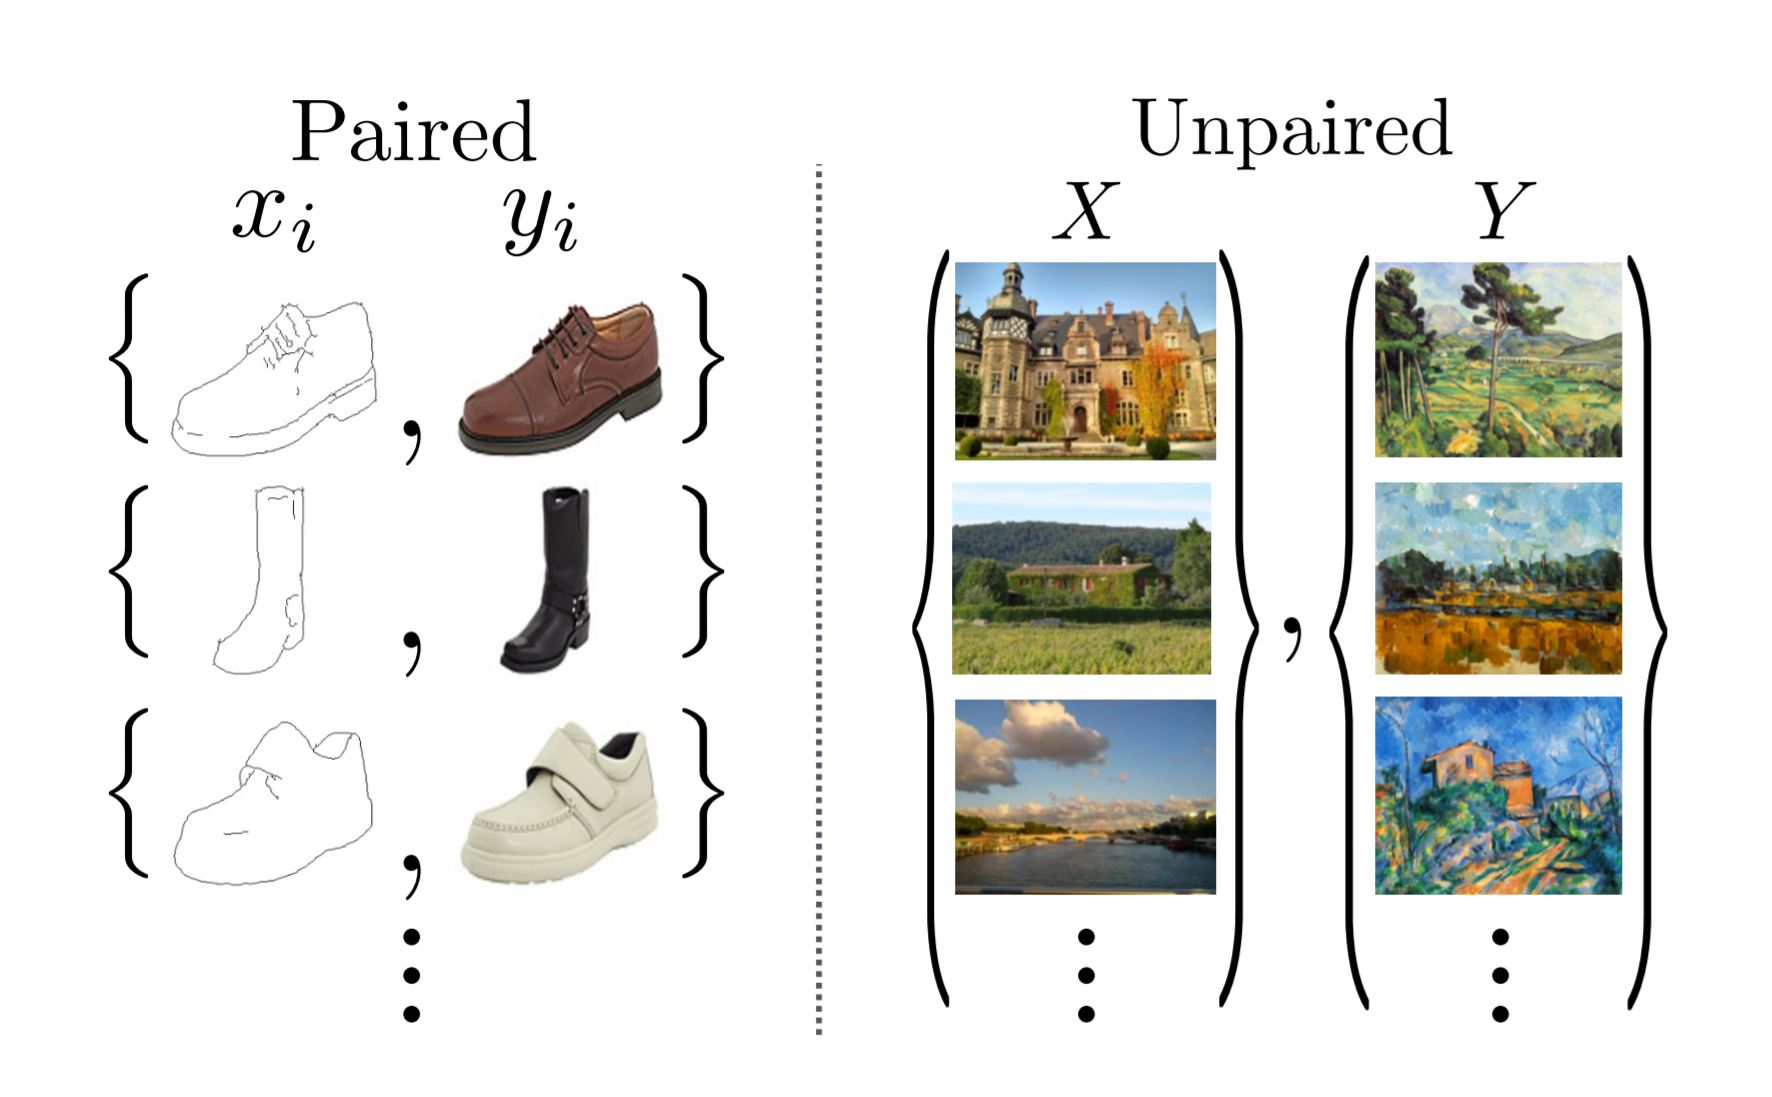
\includegraphics[width=0.8\columnwidth]{img_translation.JPG}
    \caption{Unpaired image-to-image translation}
    \label{fig:s=unpaired-img-to-img}
\end{figure}

Mapping the image to target domain is done using a generator network and the quality of this generated image is improved by pitching the generator against a discrimintor (as described below).

\subsection*{Adversarial Networks}
\qquad We have a generator network and discriminator network playing against each other. The generator tries to produce samples from the desired distribution and the discriminator tries to predict if the sample is from the actual distribution or produced by the generator. The generator and discriminator are trained jointly. The effect this has is that eventually the generator learns to approximate the underlying distribution completely and the discriminator is left guessing randomly.

\subsection*{Cycle-Consistent}
 The above adversarial method of training has a problem though. Quoting the authors of the original paper \cite{zhu2017unpaired}:

"Adversarial training can, in theory, learn mappings $G$ and $F$ that produce outputs identically distributed as target domains $Y$ and $X$ respectively. However, with large enough capacity, a network can map the same set of input images to any random permutation of images in the target domain, where any of the learned mappings can induce an output distribution that matches the target distribution. Thus, an adversarial loss alone cannot guarantee that the learned function can map an individual input $x_i$ to a desired output $y_i$."

To regularize the model, the authors introduce the constraint of cycle-consistency if we transform from source distribution to target and then back again to source distribution, we should get samples from our source distribution.

\subsection{Network Architecture}
In a paired dataset, every image, say $img_A$, is manually mapped to some image, say $img_B$, in target domain, such that they share various features. Features that can be used to map an image $(img_A/img_B)$ to its correspondingly mapped counterpart $(img_B/img_A)$. Basically, pairing is done to make input and output share some common features. This mapping defines meaningful transformation of an image from one damain to another domain. So, when we have paired dataset, generator must take an input, say $input_A$, from domain $D_A$ and map this image to an output image, say $gen_B$, which must be close to its mapped counterpart. But we don't have this luxury in unpaired dataset, there is no pre-defined meaningful transformation that we can learn, so, we will create it. We need to make sure that there is some meaningful relation between input image and generated image. So, authors tried to enforce this by saying that Generator will map input image $(input_A)$ from domain $D_A$ to some image in target domain $D_B$, but to make sure that there is meaningful relation between these images, they must share some feature, features that can be used to map this output image back to input image, so there must be another generator that must be able to map back this output image back to original input. So, we can see this condition defining a meaningful mapping between $input_A$ and $gen_B$.

In a nutshell, the model works by taking an input image from domain $D_A$ which is fed to our first generator $Generator_A\to_B$ whose job is to transform a given image from domain $D_A$ to an image in target domain $D_B$. This new generated image is then fed to another generator $Generator_B\to_A$ which converts it back into an image, $Cyclic_A$, from our original domain $D_A$ (think of autoencoders, except that our latent space is $D_t$). And as we discussed in above paragraph, this output image must be close to original input image to define a meaningful mapping that is absent in unpaired dataset.

\begin{figure}[H]
    \centering
    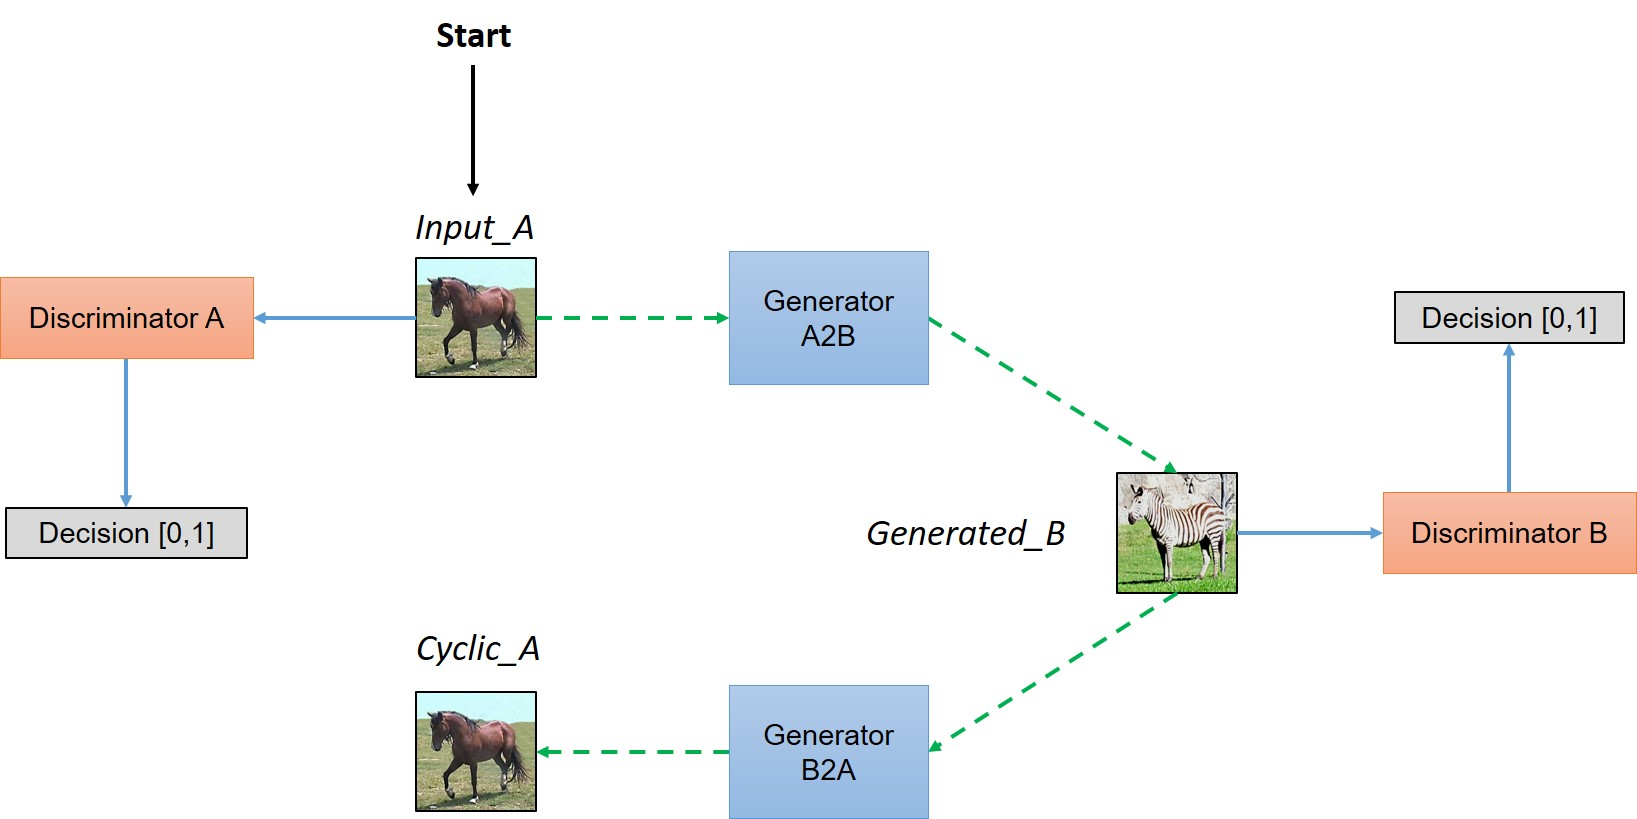
\includegraphics[width=0.8\columnwidth]{simplified_cyclegan_1.jpg}
    \par\noindent\rule{0.8\columnwidth}{0.4pt}
    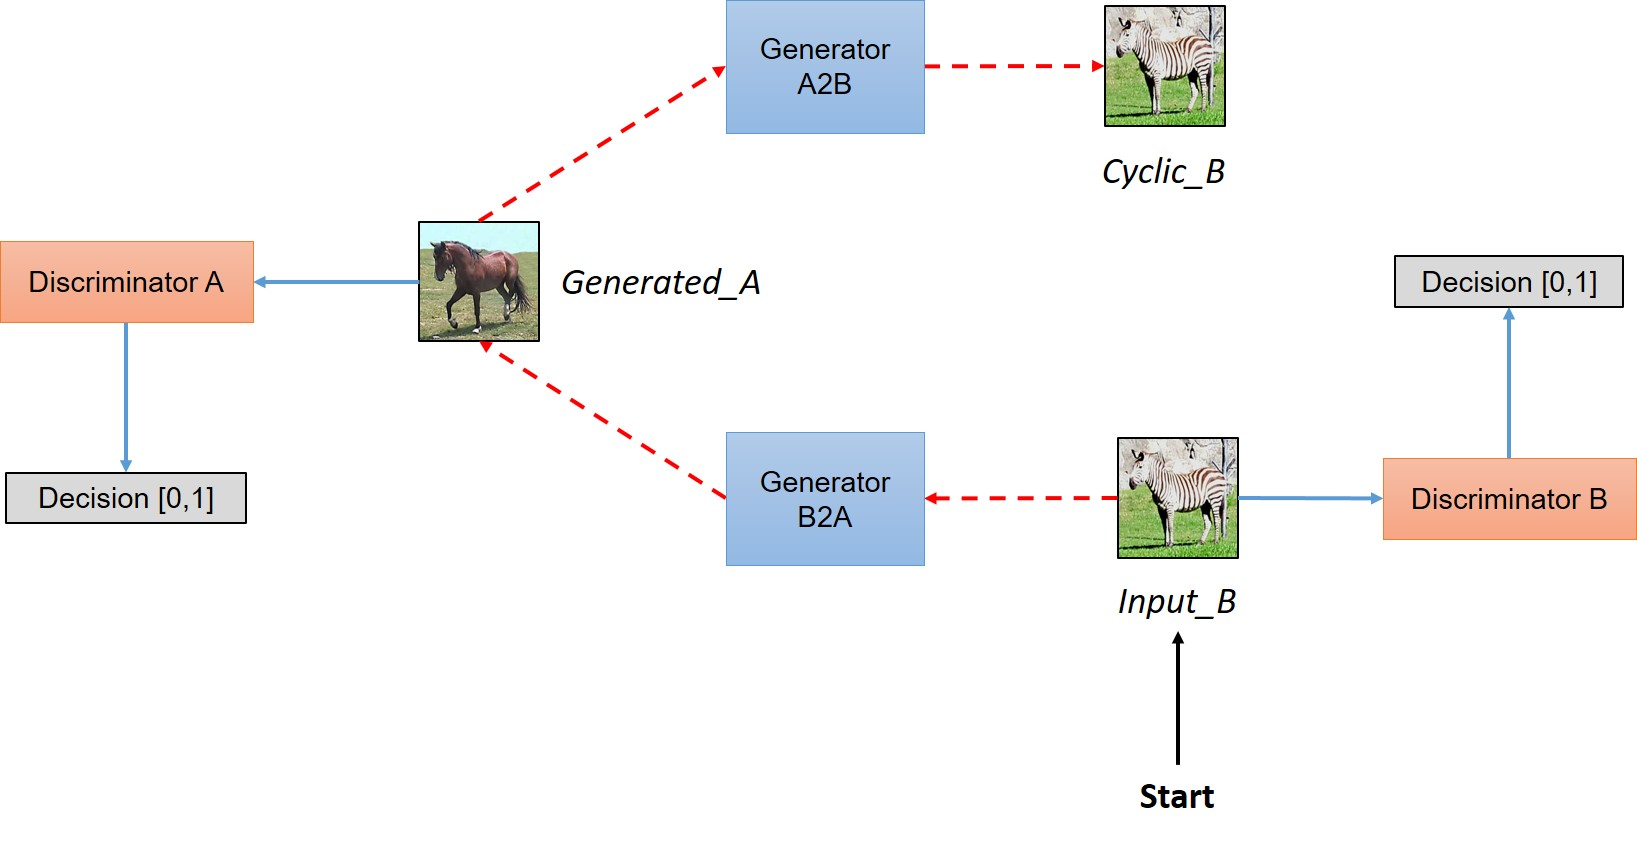
\includegraphics[width=0.8\columnwidth]{simplified_cyclegan_2.jpg}
    \caption{Simplified view of CycleGAN architecture }
    \label{fig:s=simple_cyclegan_arc}
\end{figure}

As we can see in above figure \ref{fig:s=simple_cyclegan_arc}, two inputs are fed into each discriminator(one is original image corresponding to that domain and other is the generated image via a generator) and the job of discriminator is to distinguish between them, so that discriminator is able to defy the adversary (in this case generator) and reject images generated by it. While the generator would like to make sure that these images get accepted by the discriminator, so it will try to generate images which are very close to original images in Class $D_B$. (In fact, the generator and discriminator are actually playing a game whose Nash equilibrium is achieved when the generator's distribution becomes same as the desired distribution).

% ANALYSIS / IMPLEMENTATION
\section{CycleGAN Implementation}

\subsection{Bulding Generator}
High level structure of Generator can be viewed in the following image.

\begin{figure}[H]
    \centering
    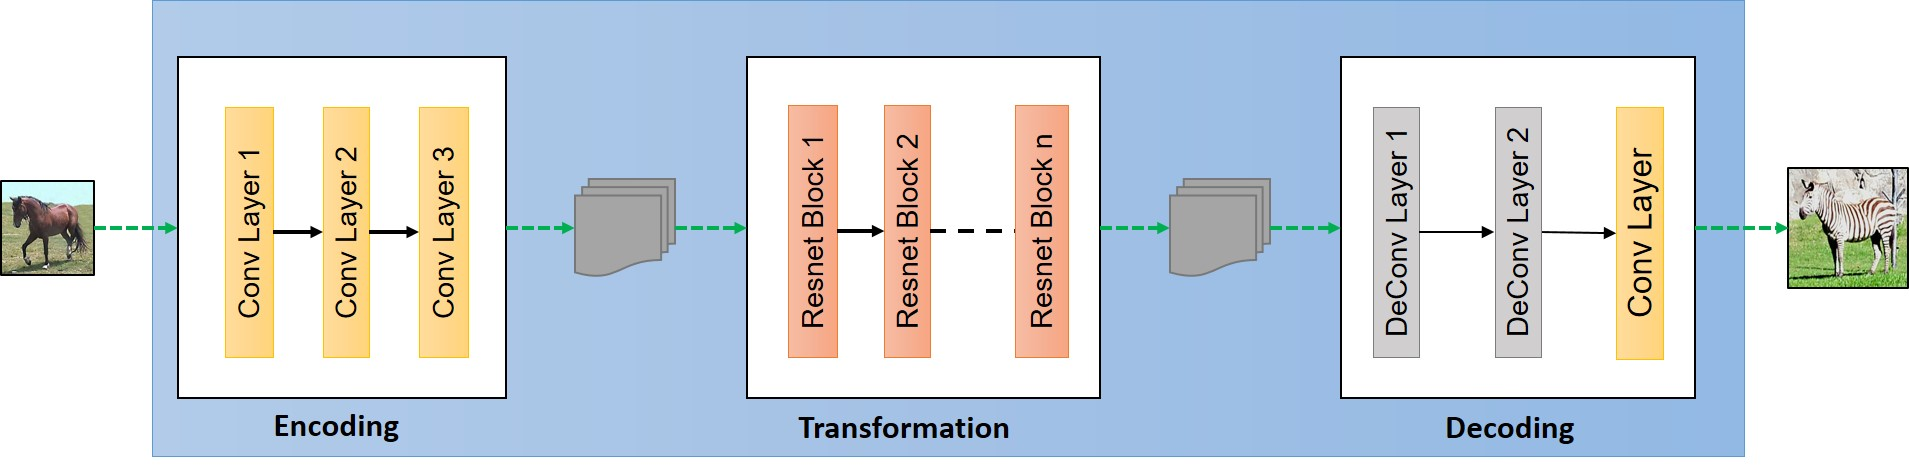
\includegraphics[width=0.8\columnwidth]{Generator.jpg}
    \caption{Generator Block}
    \label{fig:s=generator}
\end{figure}

The generator have three components:
\begin{enumerate}
  \item Encoder
  \item Transformer
  \item Decoder
\end{enumerate}
Following are the parameters we have used for the mode.

\begin{lstlisting}[language=Python]
ngf = 32 # Number of filters in first layer of generator
ndf = 64 # Number of filters in first layer of discriminator
batch_size = 1 # batch_size
pool_size = 50 # pool size
img_width = 256 # Imput image will of width 256
img_height = 256 # Input image will be of height 256
img_depth = 3 # RGB format
\end{lstlisting}

First three parameters are self explanatory and we will explain what \verb!pool_size! means in the \ref{gip} section.

\subsection{Encoding}
For the purpose of simplicity, throughout the article we will assume that the input size is $[256,256,3]$. The first step is extracting the features from an image which is done a convolution network. As input a convolution network takes an image, size of filter window that we move over input image to extract out features and the stride size to decide how much we will move filter window after each step. So the first layer of encoding looks like this:

\begin{lstlisting}[language=Python]
o_c1 = general_conv2d(input_gen, num_features=ngf, window_width=7, window_height=7, stride_width=1, stride_height=1)
\end{lstlisting}

Here \verb!input_gen! is the input image to the generator, \verb!num_features! is the number of output features we extract out of the convolution layer, which can also be seen as number of different filters used to extract different features. \verb!window_width! and \verb!window_height! denote the width and heigth of filter window that we will move accross the input image to extract features and similarly \verb!stride_width! and \verb!stride_height! defines the shift of filter patch after each step. The output \verb!o_c1! is a tensor of dimensions $[256,256,64]$ which is again passed through another convolution layer. Here, $ngf = 64$ as mentioned earlier. I have defined the \verb!general_conv2d! function.

\begin{lstlisting}[language=Python]
def general_conv2d(inputconv, o_d=64, f_h=7, f_w=7, s_h=1, s_w=1):
    with tf.variable_scope(name):
        conv = tf.contrib.layers.conv2d(inputconv, num_features, [window_width, window_height], [stride_width, stride_height], padding, activation_fn=None, weights_initializer=tf.truncated_normal_initializer(stddev=stddev), biases_initializer=tf.constant_initializer(0.0))
\end{lstlisting}

Further:

\begin{lstlisting}[language=Python]
o_c2 = general_conv2d(o_c1, num_features=64*2, window_width=3, window_height=3, stride_width=2, stride_height=2)
# o_c2.shape = (128, 128, 128)

o_enc_A = general_conv2d(o_c2, num_features=64*4, window_width=3, window_height=3, stride_width=2, stride_height=2)
# o_enc_A.shape = (64, 64, 256)
\end{lstlisting}

Each convolution layer leads to extraction of progressively higher level features. It can also be seen as compressing an image into 256 features vectors of size 64*64 each. We are now in good shape to transform this feature vector of a image in Domain DA to feature vector of an image in domain $D_B$.

To summarize, we took an image from domain $D_A$ of size $[256,256,3]$ which we fed into our encoder to get output $o_{enc}^A$ of size $[64,64,256]$.

\subsection{Transformation}
We can view these layers as combining different nearby features of an image and then based on these features making decision about how we would like to transform that feature vector/encoding $o_{enc}^A$ of an image from $D_A$ to that of $D_B$. So for this, authors have used 6 layer of resnet blocks as follow:

\begin{lstlisting}[language=Python]
o_r1 = build_resnet_block(o_enc_A, num_features=64*4)
o_r2 = build_resnet_block(o_r1, num_features=64*4)
o_r3 = build_resnet_block(o_r2, num_features=64*4)
o_r4 = build_resnet_block(o_r3, num_features=64*4)
o_r5 = build_resnet_block(o_r4, num_features=64*4)
o_enc_B = build_resnet_block(o_r5, num_features=64*4)

# o_enc_B.shape = (64, 64, 256)
\end{lstlisting}

Here $o_{enc}^B$ denotes the final output of this layer which will be of the size $[64,64,256]$. And as discussed ealier, this can be seens as the feature vector for an image in domain $D_B$.

And as we know, \verb!build_resnet_block! is a neural network layer which consists of two convolution layers where a residue of input is added to the output. This is done to ensure properties of input of previous layers are available for later layers as well, so that the their output do not deviate much from original input, otherwise the characteristics of original images will not be retained in the output and results will be very abrupt. As we discussed earlier, one of the primary aim for the task is to retain the characteristic of original input like the size and shape of the object, so residual networks are a great fit for these kind of transformations. Resnet block can be summarized in following image.

\begin{figure}[H]
    \centering
    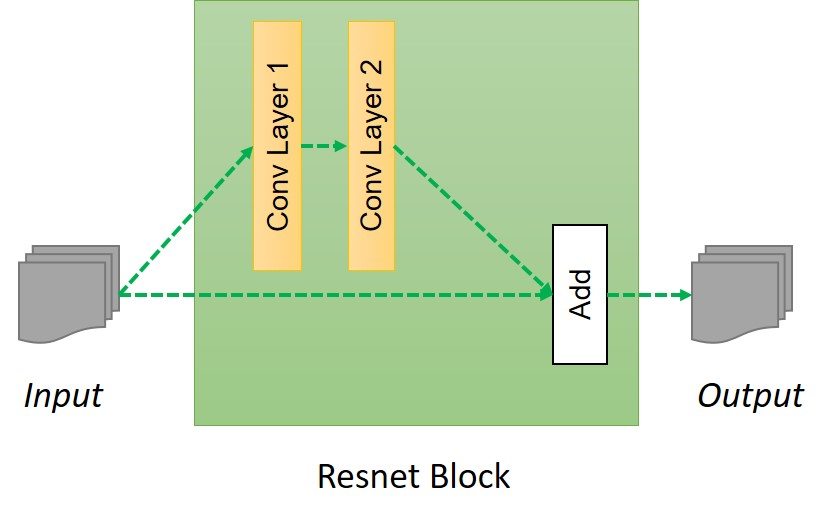
\includegraphics[width=0.8\columnwidth]{Resnet.jpg}
    \caption{Resnet Block}
    \label{fig:s=resnet}
\end{figure}

Code for Resnet block is as follow:

\begin{lstlisting}[language=Python]
def resnet_blocks(input_res, num_features):
    out_res_1 = general_conv2d(input_res, num_features, window_width=3, window_heigth=3, stride_width=1, stride_heigth=1)
    out_res_2 = general_conv2d(out_res_1, num_features, window_width=3, window_heigth=3, stride_width=1, stride_heigth=1)
    return (out_res_2 + input_res)
\end{lstlisting}

\subsection{Decoding}
Up until now we have fed a feature vector $o_{enc}^B$ into a transformation layer to get another feature vector $o_{enc}^B$ of size $[64,64,256]$.

Decoding step is exact opposite of Step 1, we will build back the low level features back from the feature vector. This is done by applying a deconvolution (or transpose convolution) layer.

\begin{lstlisting}[language=Python]
o_d1 = general_deconv2d(o_enc_B, num_features=ngf*2 window_width=3, window_height=3, stride_width=2, stride_height=2)
o_d2 = general_deconv2d(o_d1, num_features=ngf, window_width=3, window_height=3, stride_width=2, stride_height=2)
\end{lstlisting}

Finally we will convert this low level feature to image in domain $D_B$ as follow:

\begin{lstlisting}[language=Python]
gen_B = general_conv2d(o_d2, num_features=3, window_width=7, window_height=7, stride_width=1, stride_height=1)
\end{lstlisting}

So, finally we have the generate image $gen_B$ of size $[256,256,3]$ and the code for building generator can be compressed to following function:

\begin{lstlisting}[language=Python]
def build_generator(input_gen):
    o_c1 = general_conv2d(input_gen, num_features=ngf, window_width=7, window_height=7, stride_width=1, stride_height=1)
    o_c2 = general_conv2d(o_c1, num_features=ngf*2, window_width=3, window_height=3, stride_width=2, stride_height=2)
    o_enc_A = general_conv2d(o_c2, num_features=ngf*4, window_width=3, window_height=3, stride_width=2, stride_height=2)

    # Transformation
    o_r1 = build_resnet_block(o_enc_A, num_features=64*4)
    o_r2 = build_resnet_block(o_r1, num_features=64*4)
    o_r3 = build_resnet_block(o_r2, num_features=64*4)
    o_r4 = build_resnet_block(o_r3, num_features=64*4)
    o_r5 = build_resnet_block(o_r4, num_features=64*4)
    o_enc_B = build_resnet_block(o_r5, num_features=64*4)

    #Decoding
    o_d1 = general_deconv2d(o_enc_B, num_features=ngf*2 window_width=3, window_height=3, stride_width=2, stride_height=2)
    o_d2 = general_deconv2d(o_d1, num_features=ngf, window_width=3, window_height=3, stride_width=2, stride_height=2)
    gen_B = general_conv2d(o_d2, num_features=3, window_width=7, window_height=7, stride_width=1, stride_height=1)

    return gen_B
\end{lstlisting}

\subsection{Building Discriminator}
We discussed how to build a generator, however for adversarial training of the network we need to build a discriminator as well. The discriminator would take an image as an input and try to predict if it is an original or the output from the generator. Generator can be visualized in following image.

\begin{figure}[H]
    \centering
    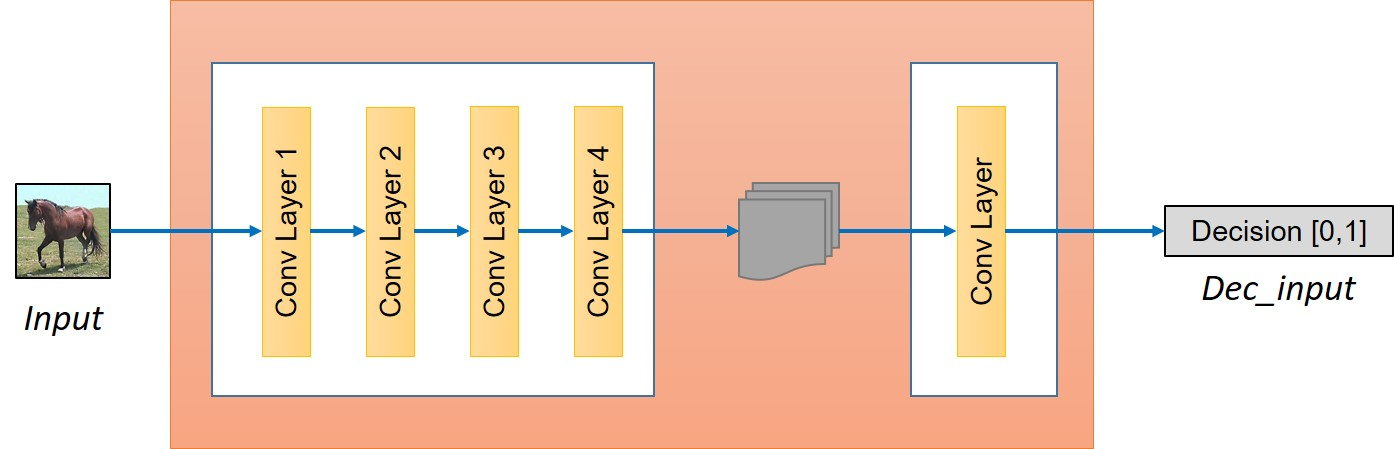
\includegraphics[width=0.8\columnwidth]{discriminator.jpg}
    \caption{Discriminator Block}
    \label{fig:s=discriminator}
\end{figure}

The discriminator is simply a convolution network in our case. First, we will extract the features from the image.

\begin{lstlisting}[language=Python]
o_c1 = general_conv2d(input_disc, ndf, f, f, 2, 2)
o_c2 = general_conv2d(o_c1, ndf*2, f, f, 2, 2)
o_enc_A = general_conv2d(o_c2, ndf*4, f, f, 2, 2)
o_c4 = general_conv2d(o_enc_A, ndf*8, f, f, 2, 2)
\end{lstlisting}

Next step is deciding whether these features belongs to that particular category or not. For that we will add a final convolution layer that produces a 1 dimensional output. Here, $ndf$ denotes the number of features in initial layer of discriminator that one can vary or experiment with to get the best result.

\begin{lstlisting}[language=Python]
decision = general_conv2d(o_c4, 1, f, f, 1, 1, 0.02)
\end{lstlisting}

We now have two main components of the model, namely Generator and Discriminator, and since we want to make this model work in both the direction i.e., from $A \to B$ and from $B \to A$, we will have two Generators, namely $Generator_{A \to B}$ and $Generator_{B \to A}$, and two Discriminators, namely $Discriminator_A$ and $Discriminator_B$.

\subsection{Bulding Model}
Before getting to loss funtion let us define the base and see how to take input, construct the model.

\begin{lstlisting}[language=Python]
input_A = tf.placeholder(tf.float32, [batch_size, img_width, img_height, img_layer], name="input_A")
input_B = tf.placeholder(tf.float32, [batch_size, img_width, img_height, img_layer], name="input_B")
\end{lstlisting}

These placeholders will act as input while defining our model as follow.

\begin{lstlisting}[language=Python]
gen_B = build_generator(input_A, name="generator_AtoB")
gen_A = build_generator(input_B, name="generator_BtoA")
dec_A = build_discriminator(input_A, name="discriminator_A")
dec_B = build_discriminator(input_B, name="discriminator_B")

dec_gen_A = build_discriminator(gen_A, "discriminator_A")
dec_gen_B = build_discriminator(gen_B, "discriminator_B")
cyc_A = build_generator(gen_B, "generator_BtoA")
cyc_B = build_generator(gen_A, "generator_AtoB")
\end{lstlisting}

Above variable names are quite intuitive in nature. $gen$ represents image generated after using corresponding Generator and $dec$ represents decision after feeding the corresponding input to the discriminator.

\subsection{Loss Function}
By now we have two generators and two discriminators. We need to design the loss function in a way which accomplishes our goal. The loss function can be seen having four parts:

\begin{enumerate}
  \item Discriminator must approve all the original images of the corresponding categories.
  \item Discriminator must reject all the images which are generated by corresponding Generators to fool them.
  \item Generators must make the discriminators approve all the generated images, so as to fool them.
  \item The generated image must retain the property of original image, so if we generate a fake image using a generator say $Generator_{A \to B}$ then we must be able to get back to original image using the another generator $Generator_{B \to A}$, it must satisfy cyclic-consistency.
\end{enumerate}

\subsection*{Discriminator Loss}
Discriminator must be trained such that recommendation for images from category A must be as close to 1, and vice versa for discriminator B. So Discriminator A would like to minimize $(Discriminator_A(a)−1)^2$ and same goes for B as well. This can be implemented as:

\begin{lstlisting}[language=Python]
D_A_loss_1 = tf.reduce_mean(tf.squared_difference(dec_A,1))
D_B_loss_1 = tf.reduce_mean(tf.squared_difference(dec_B,1))
\end{lstlisting}

Since, discriminator should be able to distinguish between generated and original images, it should also be predicting 0 for images produced by the generator, i.e. Discriminator A would like to minimize $(Discriminator_A(Generator_{B \to A}(b)))^2$. It can be calculated as follow:

\begin{lstlisting}[language=Python]
D_A_loss_2 = tf.reduce_mean(tf.square(dec_gen_A))
D_B_loss_2 = tf.reduce_mean(tf.square(dec_gen_B))

D_A_loss = (D_A_loss_1 + D_A_loss_2)/2
D_B_loss = (D_B_loss_1 + D_B_loss_2)/2
\end{lstlisting}

\subsection*{Generator Loss}
Generator should eventually be able to fool the discriminator about the authencity of it's generated images. This can done if the recommendation by discriminator for the generated images is as close to 1 as possible. So generator would like to minimize $(Discriminator_B(Generator_{A \to B}(a))−1)^2$ So the loss is:

\begin{lstlisting}[language=Python]
g_loss_B_1 = tf.reduce_mean(tf.squared_difference(dec_gen_A,1))
g_loss_A_1 = tf.reduce_mean(tf.squared_difference(dec_gen_A,1))
\end{lstlisting}

\subsection*{Cyclic Loss}
And the last one and one of the most important one is the cyclic loss that captures that we are able to get the image back using another generator and thus the difference between the original image and the cyclic image should be as small as possible.

\begin{lstlisting}[language=Python]
cyc_loss = tf.reduce_mean(tf.abs(input_A-cyc_A)) + tf.reduce_mean(tf.abs(input_B-cyc_B))
\end{lstlisting}

The complete generator loss is then:

\begin{lstlisting}[language=Python]
g_loss_A = g_loss_A_1 + 10*cyc_loss
g_loss_B = g_loss_B_1 + 10*cyc_loss
\end{lstlisting}

The multiplicative factor of 10 for \verb!cyc_loss! assigns more importance to cyclic loss than the discrimination loss.

\subsection*{All Losses}
With the loss function defined, all the is needed to train the model is to minimize the loss function w.r.t. model parameters.

\begin{lstlisting}[language=Python]
d_A_trainer = optimizer.minimize(d_loss_A, var_list=d_A_vars)
d_B_trainer = optimizer.minimize(d_loss_B, var_list=d_B_vars)
g_A_trainer = optimizer.minimize(g_loss_A, var_list=g_A_vars)
g_B_trainer = optimizer.minimize(g_loss_B, var_list=g_B_vars)
\end{lstlisting}

\subsection{Training Model}

\begin{lstlisting}[language=Python]
for epoch in range(0,100):
    # Define the learning rate schedule. The learning rate is kept
    # constant upto 100 epochs and then slowly decayed
    if(epoch < 100) :
        curr_lr = 0.0002
    else:
        curr_lr = 0.0002 - 0.0002*(epoch-100)/100

    # Running the training loop for all batches
    for ptr in range(0,num_images):

        # Train generator G_A->B
        _, gen_B_temp = sess.run([g_A_trainer, gen_B], feed_dict={input_A:A_input[ptr], input_B:B_input[ptr], lr:curr_lr})

        # We need gen_B_temp because to calculate the error in training D_B
        _ = sess.run([d_B_trainer], feed_dict={input_A:A_input[ptr], input_B:B_input[ptr], lr:curr_lr})

        # Same for G_B->A and D_A as follow
        _, gen_A_temp = sess.run([g_B_trainer, gen_A], feed_dict={input_A:A_input[ptr], input_B:B_input[ptr], lr:curr_lr})
        _ = sess.run([d_A_trainer], feed_dict={input_A:A_input[ptr], input_B:B_input[ptr], lr:curr_lr})
\end{lstlisting}

As we can see in above training function that one by one we are calling trainers corresponding to different Dicriminators and Generators. For training them, we need to feed traing images and learning rate of the optimizer. Since, we have \verb!batch_size = 1!, so, \verb!num_batches = num_images!.

Since, we are nearly done with the code, below is look at the default parameters that we took to train the model.

\subsection*{Generated Image Pool} \label{gip}
Calculating the discriminator loss for each generated image would be computationally prohibitive. To speed up training we store a collection of previously generated images for each domain and to use only one of these images for calculating the error. First, fill the \verb!image_pool! one by one until its full and after that randomly replace an image from the pool and store the latest one and use the replaced image for training in that iteration.

\begin{lstlisting}[language=Python]
def image_pool(self, num_gen, gen_img, gen_pool):
    if(num_gen < pool_size):
        gen_img_pool[num_gen] = gen_img
        return gen_img
    else :
        p = random.random()
        if p > 0.5:
            # Randomly selecting an id to return for calculating the discriminator loss
            random_id = random.randint(0,pool_size-1)
            temp = gen_img_pool[random_id]
            gen_pool[random_id] = gen_img
            return temp
        else :
            return gen_img
\end{lstlisting}

\begin{lstlisting}[language=Python]
gen_image_pool_A = tf.placeholder(tf.float32, [batch_size, img_width, img_height, img_layer], name="gen_img_pool_A")
gen_image_pool_B = tf.placeholder(tf.float32, [batch_size, img_width, img_height, img_layer], name="gen_img_pool_B")

gen_pool_rec_A = build_gen_discriminator(gen_image_pool_A, "d_A")
gen_pool_rec_B = build_gen_discriminator(gen_image_pool_B, "d_B")

# Also the discriminator loss will change as follow

D_A_loss_2 = tf.reduce_mean(tf.square(gen_pool_rec_A))
D_A_loss_2 = tf.reduce_mean(tf.square(gen_pool_rec_A))
\end{lstlisting}

% CONCLUSION
\section{Results and Conclusions}
I ran the model for \href{https://people.eecs.berkeley.edu/~taesung_park/CycleGAN/datasets/horse2zebra.zip}{horse2zebra} dataset but because of the lack of resources, i just ran the model for 100 epochs and got following results.

\begin{figure}[H]
    \centering
    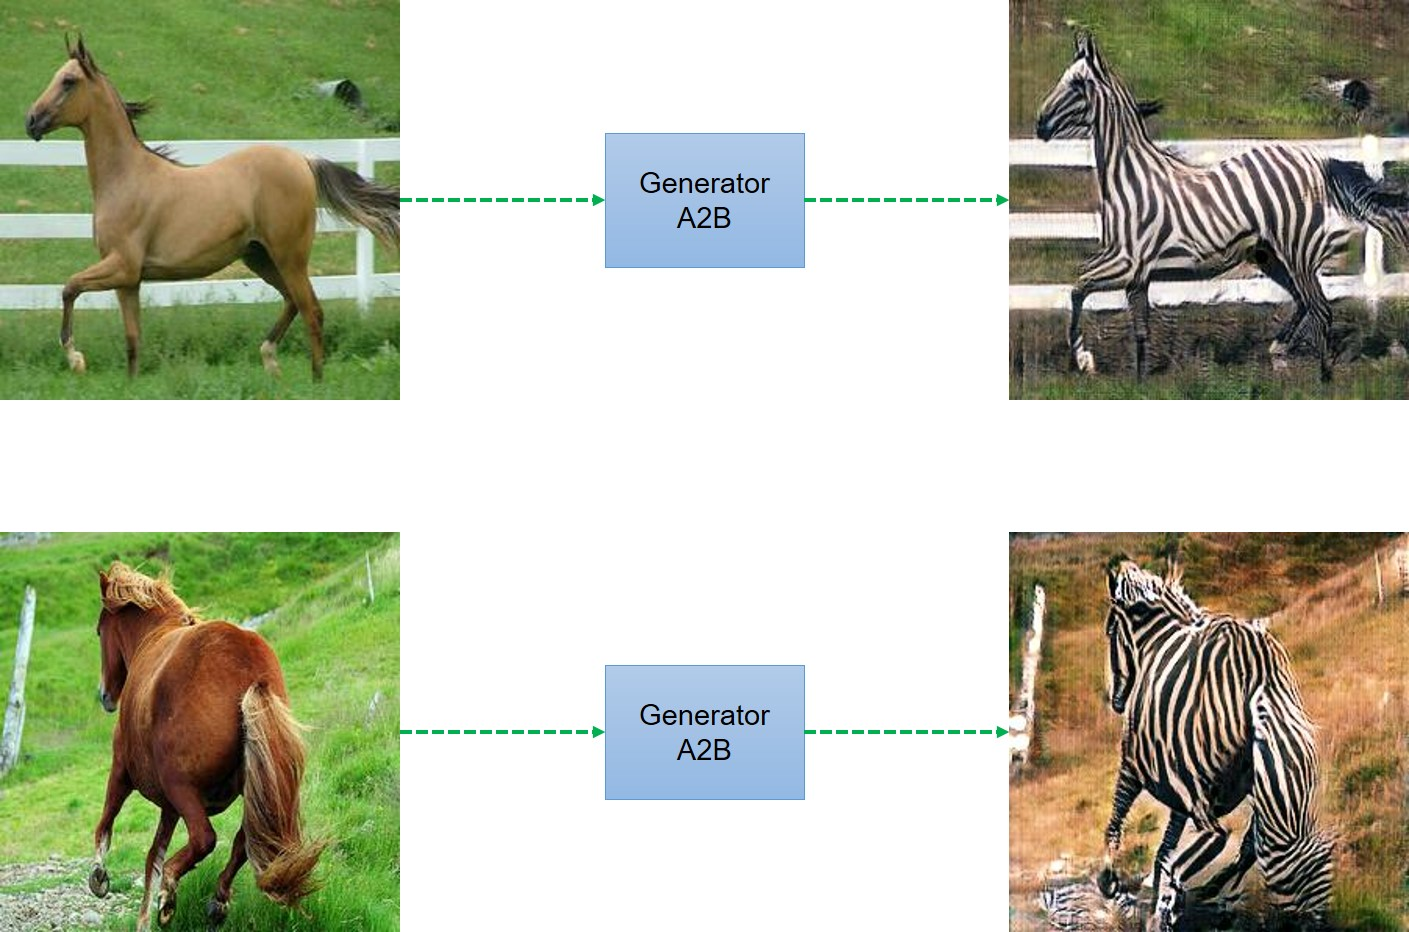
\includegraphics[width=0.8\columnwidth]{Results.jpg}
    \caption{Result}
    \label{fig:s=result}
\end{figure}

During training i noticed that the ouput results were sensitive to initialization. We might notice background color being reversed as in following image. This effect can be observed only after 10-20 epochs and you can try to run the code again. I also think that this model is not good fit to change the shape of object. I tried to run the model for converting a men's face to a look alike women's face. For that i used celebA dataset but the results are not good and images produced are quite distorted.

% references
\bibliographystyle{plain} % We choose the "plain" reference style
\bibliography{refs} % Entries are in the refs.bib file

\end{document}